\chapter{Bauteile}
\label{kap:format-bauteile}

\section{Allgemeines}

Jedes Bauteil ist ein Objekt in der Liste \code{components}:

\begin{json}
{ "type": "R", "name": "R1", "nodes": ["in", "out"], "value": "4.7k" }
\end{json}

\begin{description}[style=nextline,leftmargin=2em]
  \item[\code{type}] der SPICE-Buchstabe oder der lange Name (\code{"R"} oder
    \code{"resistor"}); Groß- und Kleinschreibung egal.
  \item[\code{name}] optional, aber nötig für \code{i(...)}, als Quelle eines
    DC-Sweeps, als Steuerung gesteuerter Quellen und für die Kopplung.
    Bauteile ohne Namen bekommen einen aus Typ und Position (\code{V2}).
  \item[\code{nodes}] die Knoten in der Reihenfolge der Tabelle unten.
  \item[weitere Schlüssel] die Werte und Parameter des Bauteils.
\end{description}

\section{Übersicht}

\begin{longtable}{@{}P{2.6cm}P{3.6cm}P{2.6cm}P{5.0cm}@{}}
  \toprule
  \code{type} & Bauteil & \code{nodes} & Parameter \\
  \midrule
  \endhead
  \bottomrule
  \endfoot
  \code{R}, \code{resistor} & Widerstand & a, b & \code{value}; \code{"noise": false} ohne thermisches Rauschen \\
  \code{C}, \code{capacitor} & Kondensator & a, b & \code{value}, \code{ic} (Spannung a$-$b bei $t=0$) \\
  \code{L}, \code{inductor} & Spule & a, b & \code{value}, \code{ic} (Strom a$\to$b bei $t=0$) \\
  \code{V}, \code{vsource} & Spannungsquelle & $+$, $-$ & \code{dc}, \code{wave}, \code{ac}, \code{acphase} \\
  \code{I}, \code{isource} & Stromquelle & von, nach & \code{dc}, \code{wave}, \code{ac}, \code{acphase} \\
  \code{E}, \code{vcvs} & spannungsgesteuerte Spannungsquelle & $+$, $-$, Steuer$+$, Steuer$-$ & \code{gain} \\
  \code{G}, \code{vccs} & spannungsgesteuerte Stromquelle & von, nach, Steuer$+$, Steuer$-$ & \code{gm} \\
  \code{F}, \code{cccs} & stromgesteuerte Stromquelle & von, nach & \code{control}, \code{gain} \\
  \code{H}, \code{ccvs} & stromgesteuerte Spannungsquelle & $+$, $-$ & \code{control}, \code{r} \\
  \code{B}, \code{behavioral} & Verhaltensquelle & $+$, $-$ & genau eines von \code{i}, \code{v}, \code{q}, \code{phi} \\
  \code{K}, \code{coupling} & magnetische Kopplung & – & \code{inductors}, \code{k} \\
  \code{T}, \code{tline} & Leitung & Tor 1 ($+$, $-$), Tor 2 ($+$, $-$) & \code{z0}, \code{td} oder \code{f}/\code{nl} oder \code{l}/\code{c}/\code{len}; Verluste \code{r}, \code{g}, \code{segments} \\
  \code{S}, \code{switch} & idealer Schalter & a, b [, Steuer$+$, Steuer$-$] & \code{control}, \code{vt}, \code{vh}, \code{ron}, \code{roff}, \code{initial} \\
  \code{ideal_diode} & ideale Diode & Anode, Kathode & \code{vf}, \code{ron}, \code{roff} \\
  \code{D}, \code{diode} & Diode & Anode, Kathode & \code{model} oder Parameter (Kapitel~\ref{kap:format-modelle}) \\
  \code{Q}, \code{npn}, \code{pnp} & Bipolartransistor & C, B, E & \code{model} oder Parameter \\
  \code{J}, \code{njf}, \code{pjf} & Sperrschicht-FET & D, G, S & \code{model} oder Parameter \\
  \code{M}, \code{nmos}, \code{pmos} & MOSFET & D, G, S [, Bulk] & \code{model}, \code{w}, \code{l}, Parameter \\
  \code{X}, \code{subcircuit} & Instanz einer Teilschaltung & in der Reihenfolge der \code{ports} & \code{subcircuit}, \code{parameters} \\
\end{longtable}

\section{Widerstand, Kondensator, Spule}

\begin{json}
{ "type": "R", "name": "R1", "nodes": ["a", "b"], "value": "10k" },
{ "type": "C", "name": "C1", "nodes": ["b", "0"], "value": "100n", "ic": 2.5 },
{ "type": "L", "name": "L1", "nodes": ["b", "c"], "value": "1m",   "ic": "10m" }
\end{json}

\code{value} darf ein Ausdruck aus Parametern sein. \code{ic} ist der
Anfangswert für eine Transientenanalyse mit \code{"uic": true}
(Abschnitt~\ref{sec:tran}). Widerstände rauschen thermisch; mit
\code{"noise": false} nicht (nützlich für Hilfswiderstände in
Makromodellen). Nichtlineare Widerstände, Kondensatoren und Spulen
entstehen mit der Verhaltensquelle \code{B}.

\section{Unabhängige Quellen}
\label{sec:quellen}

\begin{json}
{ "type": "V", "name": "Vcc", "nodes": ["vcc", "0"], "dc": 12 },
{ "type": "V", "name": "Vin", "nodes": ["in", "0"], "dc": 0, "ac": 1,
  "wave": { "type": "sin", "amplitude": "10m", "freq": "1k" } },
{ "type": "I", "name": "Ib", "nodes": ["0", "b"], "dc": "10u" }
\end{json}

\begin{itemize}
  \item \code{dc} ist der Wert für Arbeitspunkt, DC-Sweep und den
    Arbeitspunkt der AC-Analyse. Ohne \code{dc} gilt dort der Wert von
    \code{wave} bei $t=0$.
  \item \code{wave} beschreibt den Zeitverlauf für die Transientenanalyse.
  \item \code{ac} (Amplitude, Standard 0) und \code{acphase} (Grad) sind die
    Kleinsignalanregung der AC-Analyse.
\end{itemize}

\begin{center}
\begin{tabularx}{\textwidth}{@{}lL@{}}
  \toprule
  \code{wave.type} & Parameter \\
  \midrule
  \code{sin} & \code{offset}, \code{amplitude}, \code{freq}, \code{delay}, \code{damping} (1/s), \code{phase} (Grad) \\
  \code{pulse} & \code{v1}, \code{v2}, \code{delay}, \code{rise}, \code{fall}, \code{width}, \code{period} \\
  \code{pwl} & \code{points}: \code{[[t0, v0], [t1, v1], ...]} \\
  \code{dc} & \code{value} \\
  \bottomrule
\end{tabularx}
\end{center}

\paragraph{Sinus.}
$v(t) = \mathit{offset} + \mathit{amplitude}\cdot
e^{-\mathit{damping}\,(t-\mathit{delay})}
\sin\bigl(2\pi\,\mathit{freq}\,(t-\mathit{delay}) + \mathit{phase}\bigr)$
für $t \geq \mathit{delay}$, davor der Wert bei $t = \mathit{delay}$. Sinusquellen
begrenzen die Schrittweite auf ein Zwanzigstel ihrer Periode.

\paragraph{Puls.}
Von \code{v1} nach \code{delay} in der Zeit \code{rise} auf \code{v2}, dort
\code{width} lang, in \code{fall} zurück. Mit \code{period} wiederholt sich
das, ohne \code{period} ist es ein Einzelpuls. \code{rise} und
\code{fall} sind ohne Angabe 0,1\,\% der Periode. Die Ecken des Pulses
werden als Haltepunkte exakt getroffen.

\paragraph{Stückweise linear.}
\code{points} sind Paare aus Zeit und Wert; zwischen ihnen wird linear
interpoliert, nach dem letzten der letzte Wert gehalten. Jede Stützstelle
ist ein Haltepunkt.

\paragraph{Vorzeichen.}
\code{i(V1)} ist der Strom vom Plus-Knoten \emph{durch die Quelle} zum
Minus-Knoten – also negativ, solange die Quelle Leistung abgibt (wie in
SPICE). Eine Stromquelle treibt ihren Strom vom ersten Knoten durch die
Quelle zum zweiten; \code{["0", "b"]} speist also in den Knoten \code{b}.

\section{Gesteuerte Quellen}

\begin{json}
{ "type": "E", "name": "E1", "nodes": ["out", "0", "inp", "inn"], "gain": 1e5 },
{ "type": "G", "name": "G1", "nodes": ["0", "x", "a", "b"], "gm": "1m" },
{ "type": "F", "name": "F1", "nodes": ["0", "y"], "control": "Vsense", "gain": 100 },
{ "type": "H", "name": "H1", "nodes": ["z", "0"], "control": "L1", "r": "1k" }
\end{json}

\code{E} und \code{G} werden von der Spannung zwischen den Steuerknoten
gesteuert, \code{F} und \code{H} vom Strom eines Bauteils mit Zweigstrom:
einer Spannungsquelle oder einer Spule (\code{control}). Um einen beliebigen
Strom zu messen, schaltet man eine Spannungsquelle mit 0\,V in Reihe.
Nichtlineare oder mehrfach gesteuerte Quellen sind Verhaltensquellen.

\section{Verhaltensquelle B}
\label{sec:bquelle}

Die Verhaltensquelle ist das vielseitigste Bauteil: Strom, Spannung, Ladung
oder Fluss sind ein beliebiger Ausdruck aus Knotenspannungen, Strömen,
Variablen, Parametern, Tabellen und der Zeit.

\begin{description}[style=nextline,leftmargin=2em]
  \item[{\code{"i": "..."}}]
    Strom vom Plus-Knoten durch das Bauteil zum Minus-Knoten. Ein
    nichtlinearer Widerstand: \code{"i": "1e-3*tanh(v(a,b)/0.1)"}.
  \item[{\code{"v": "..."}}]
    Spannung zwischen den Knoten; das Bauteil hat einen eigenen Zweigstrom
    \code{i(Name)}.
  \item[{\code{"q": "..."}}]
    Gespeicherte Ladung; der Strom ist ihre Zeitableitung. Ein
    spannungsabhängiger Kondensator: \code{"q": "C0*v(a,b) + C1*v(a,b)^2"}.
  \item[{\code{"phi": "..."}}]
    Magnetischer Fluss; die Spannung ist seine Zeitableitung. Der Ausdruck
    hängt in der Regel vom eigenen Strom ab. Eine sättigende Drossel:
    \code{"phi": "L0*Isat*tanh(i(L1)/Isat)"}.
\end{description}

Die Ableitungen nach allen vorkommenden Größen bildet esim selbst; auch in
der AC- und Rauschanalyse ist die Verhaltensquelle deshalb richtig
linearisiert. Vergleiche und \code{if} in Verhaltensquellen schalten als
Ereignis (Abschnitt~\ref{sec:ereignisse}). Verhaltensquellen rauschen
nicht.

\section{Magnetische Kopplung K}

\begin{json}
{ "type": "L", "name": "L1", "nodes": ["p1", "p2"], "value": "10m" },
{ "type": "L", "name": "L2", "nodes": ["s1", "s2"], "value": "1m" },
{ "type": "K", "name": "K1", "inductors": ["L1", "L2"], "k": 0.99 }
\end{json}

Die Kopplung verbindet zwei Spulen mit der Gegeninduktivität
$M = k\sqrt{L_1 L_2}$, $-1 < k < 1$. Der erste Knoten jeder Spule trägt den
Wicklungspunkt. Ein Übertrager mit dem Übersetzungsverhältnis $n$ hat
$L_2 = n^2 L_1$.

\section{Schalter S}
\label{sec:schalter}

\begin{json}
{ "type": "S", "name": "S1", "nodes": ["in", "sw", "gate", "0"], "vt": 0.5 },
{ "type": "S", "name": "S2", "nodes": ["a", "b"], "control": "i(L1)", "vt": "1", "vh": "0.1" }
\end{json}

\begin{itemize}
  \item Mit vier Knoten steuert die Spannung zwischen den Steuerknoten (wie
    in SPICE), mit zwei Knoten ein beliebiger Ausdruck in \code{control}:
    \code{"v(gate)"}, \code{"i(L1)"}, \code{"sin(2*pi*50*t)"}, eine
    Variable \dots
  \item Der Schalter schließt, wenn die Steuergröße über $v_t + v_h$
    steigt, und öffnet, wenn sie unter $v_t - v_h$ fällt (\code{vt}
    Schwelle, \code{vh} halbe Breite der Hysterese, beide Standard 0).
  \item \code{ron} (Standard 1\,m\ohm) und \code{roff} (Standard
    1\,G\ohm) sind die Widerstände in beiden Stellungen.
  \item \code{"initial": "on"} legt die Stellung fest, solange die
    Steuergröße beim Start innerhalb der Hysterese liegt.
\end{itemize}

\section{Ideale Diode}

\begin{json}
{ "type": "ideal_diode", "name": "D1", "nodes": ["0", "sw"], "vf": 0.4 }
\end{json}

Sie sperrt unterhalb der Flussspannung \code{vf} (Standard 0) mit
\code{roff} und leitet darüber mit der Steigung $1/r_\text{on}$. Im
Unterschied zur Diode \code{D} hat sie keine Exponentialkennlinie und keine
Ladung; sie ist für Leistungselektronik und Gleichrichter gedacht, wenn nur
das Schaltverhalten interessiert.

Schalter und ideale Dioden schalten als Ereignis: Der Umschaltzeitpunkt
wird exakt bestimmt. Hängen mehrere voneinander ab – ein Schalter öffnet an
einer Spule, also muss die Freilaufdiode leiten –, stellen sie sich im
selben Zeitpunkt gemeinsam ein, ohne künstliche Spannungsspitze.

\begin{figure}[htbp]
  \centering
  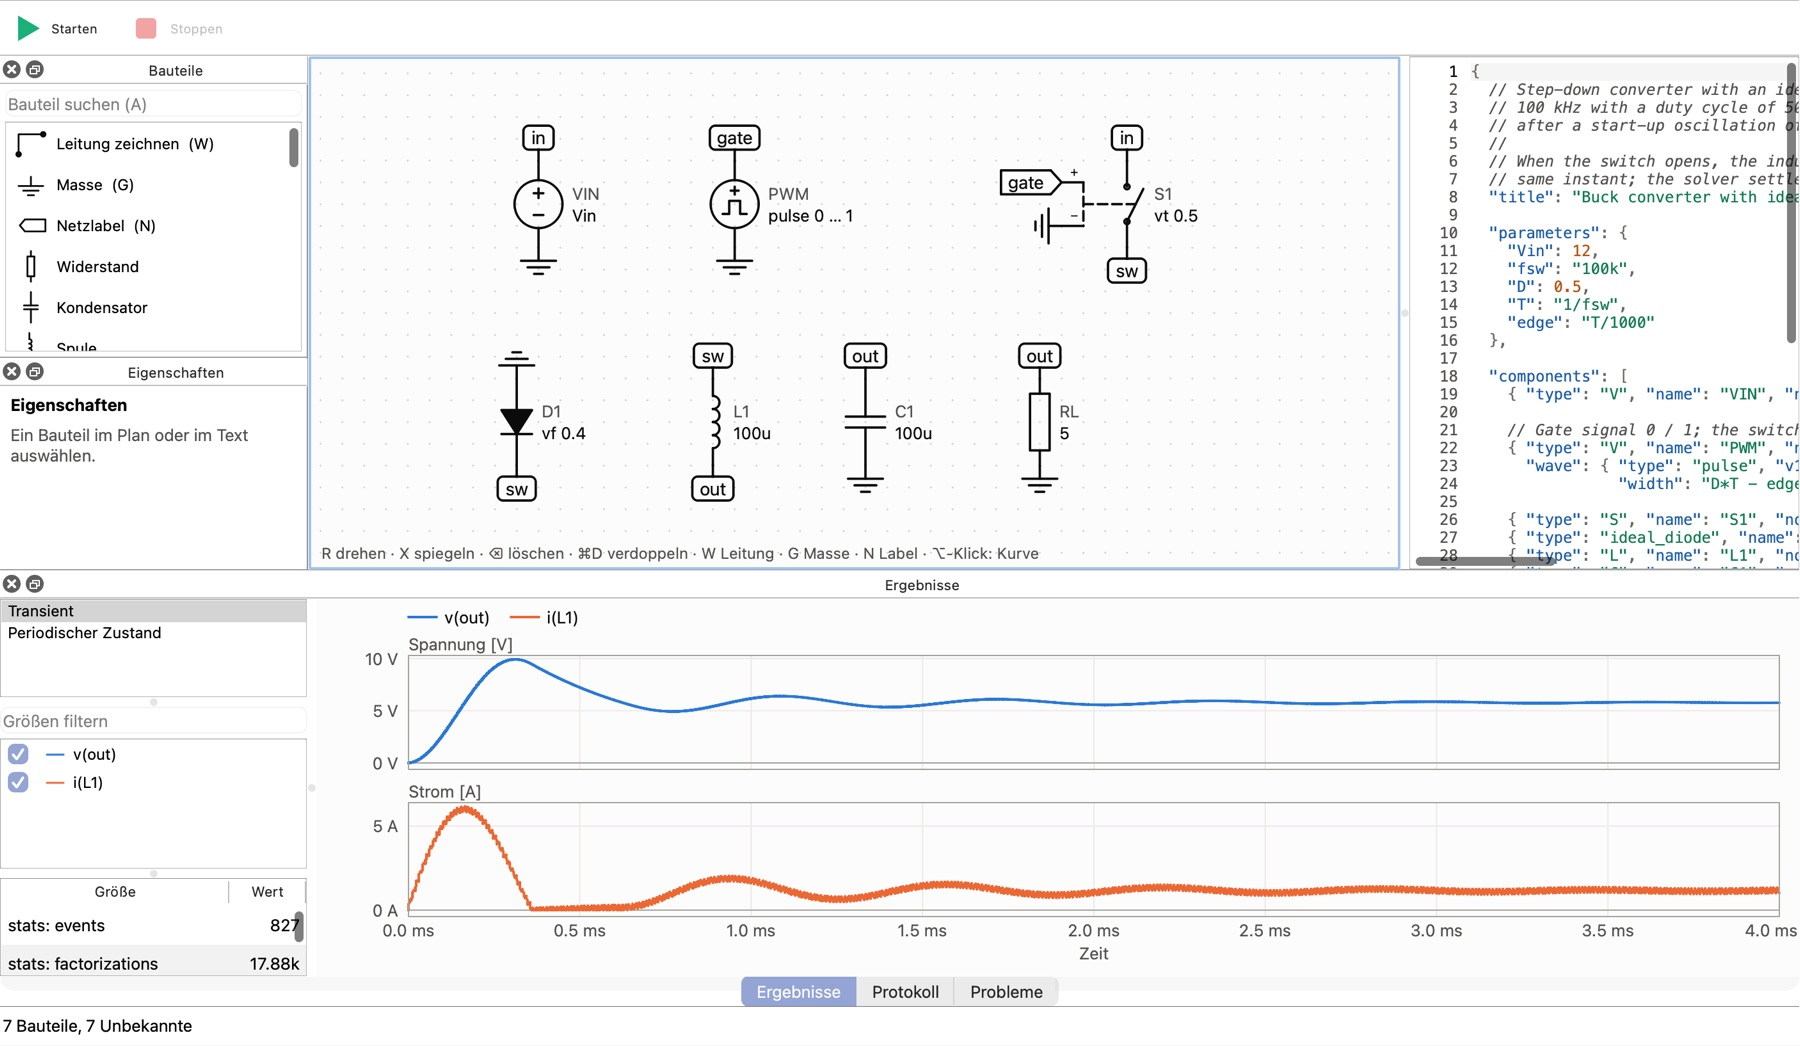
\includegraphics[width=\textwidth]{buck_converter.jpg}
  \caption{Tiefsetzsteller mit idealem Schalter und idealer Diode
    (\code{examples/buck_converter.json}): Einschwingen von
    Ausgangsspannung und Spulenstrom, 827 Schaltereignisse.}
  \label{abb:buck}
\end{figure}

\section{Leitungen T}
\label{sec:leitung}

\begin{json}
{ "type": "T", "name": "T1", "nodes": ["a", "0", "b", "0"], "z0": 50, "td": "5n" },
{ "type": "T", "name": "T2", "nodes": ["c", "0", "d", "0"],
  "l": "250n", "c": "100p", "r": 0.2, "g": 0, "len": 3 }
\end{json}

\begin{itemize}
  \item \textbf{Verlustlos}: Wellenwiderstand \code{z0} und Laufzeit
    \code{td}; alternativ wie in SPICE \code{f} und \code{nl} (Laufzeit
    $= \mathit{nl}/f$), oder Induktivitätsbelag \code{l} und
    Kapazitätsbelag \code{c} je Länge mit der Länge \code{len}.
  \item In der Zeitsimulation wird die Vorgeschichte der Wellen an beiden
    Toren gespeichert; kein Schritt ist länger als \code{td}, und Flanken
    setzen an ihrer Ankunftszeit einen Haltepunkt. Im Arbeitspunkt ist die
    Leitung eine Verbindung, in der AC-Analyse wirkt die Laufzeit exakt als
    Phasendrehung.
  \item \textbf{Verlustbehaftet}: Mit Längswiderstand \code{r} und
    Querleitwert \code{g} je Länge wird die Leitung in verlustlose
    Abschnitte geteilt, zwischen denen die Verluste sitzen. Die Laufzeit
    bleibt exakt; der Fehler fällt mit dem Quadrat der Abschnittszahl. Ohne
    \code{segments} wird sie so gewählt, dass auf jeden Abschnitt höchstens
    ein Zehntel von $Z_0$ entfällt. Der Skineffekt ist nicht modelliert.
  \item \code{i(T1)} ist der Strom in Tor~1.
\end{itemize}

\section{Halbleiter}

Dioden, Bipolartransistoren, JFETs und MOSFETs bekommen ihre Parameter
entweder direkt am Bauteil oder über \code{"model": "<Name>"} aus
\code{models}; Angaben am Bauteil überschreiben das Modell:

\begin{json}
{ "type": "M", "name": "M1", "nodes": ["d", "g", "0", "0"], "model": "n18",
  "w": "2u", "l": "0.18u" }
\end{json}

Die Polarität eines Transistors folgt aus dem \code{type} des Bauteils
(\code{npn}, \code{pmos}, \dots) oder des Modells. Ein MOSFET mit drei Knoten
hat seinen Bulk an der Source. Die Modelle beschreibt
Kapitel~\ref{kap:format-modelle}.
